\chapter{Magnolia IDE} \label{cha:ide}

This section will discuss the new Magnolia \gls{ide}, the different users of the
\gls{ide}, and their possible experiences which was under consideration when
developing the application.

\section{User Perspectives}

This application has to consider different users.

\subsection{Module Developer}

Being a zero core application; all functionality comes from modules, the module
developer experience is the most important.

\subsubsection{Language Agnostic Modules}

The largest limiting factor in module oriented applications, is the
\textit{language barrier} Most applications limit what language one can extend
an application with, like in "Visual Studio Code", where its
JavaScript/HTML/CSS. Or IntelliJ, where one can use Java or Kotlin. But what
does language agnostic mean in the context of programming languages? It is, and
always will be C. Any \textit{serious} language has some form of C-\gls{abi}.
So, for a module application to be Language Agnostic, it must be able to invoke
C Modules.

\begin{figure}
  \begin{center}
    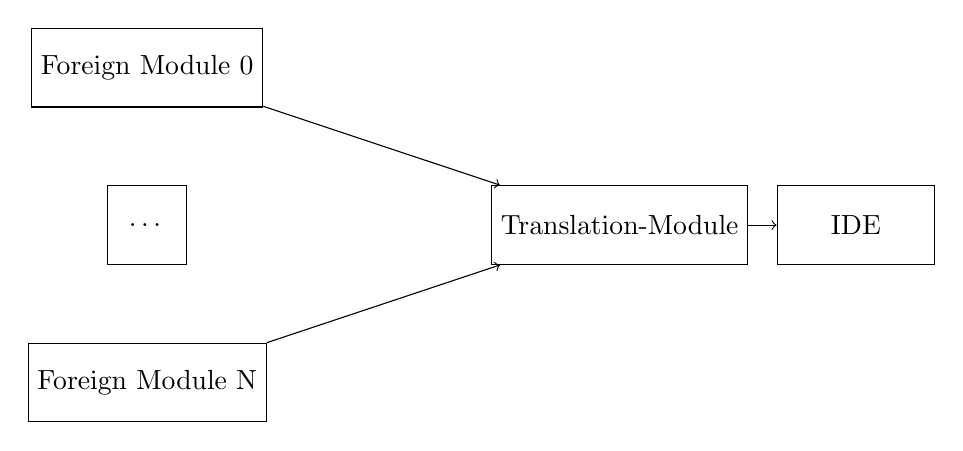
\begin{tikzpicture}
  % Nodes
  \node (p-0) [rectangle, draw, minimum height=1cm, minimum width=2cm] at (-6, 2) {Foreign Module 0};
  \node (dots) [rectangle, draw, minimum height=1cm, minimum width=1cm] at (-6, 0) {\dots};
  \node (p-n) [rectangle, draw, minimum height=1cm, minimum width=2cm] at (-6, -2) {Foreign Module N};
  \node (m) [rectangle, draw, minimum height=1cm, minimum width=2cm] at (0, 0) {Translation-Module};
  \node (i) [rectangle, draw, minimum height=1cm, minimum width=2cm] at (3, 0) {IDE};
  % Arrow
  \draw[->] (m) -- (i);
  \draw[->] (p-0) -- (m);
  \draw[->] (p-n) -- (m);
  % Header
\end{tikzpicture}

  \end{center}
  \label{fig:fm1}
\end{figure}

\begin{figure}
  \begin{center}
    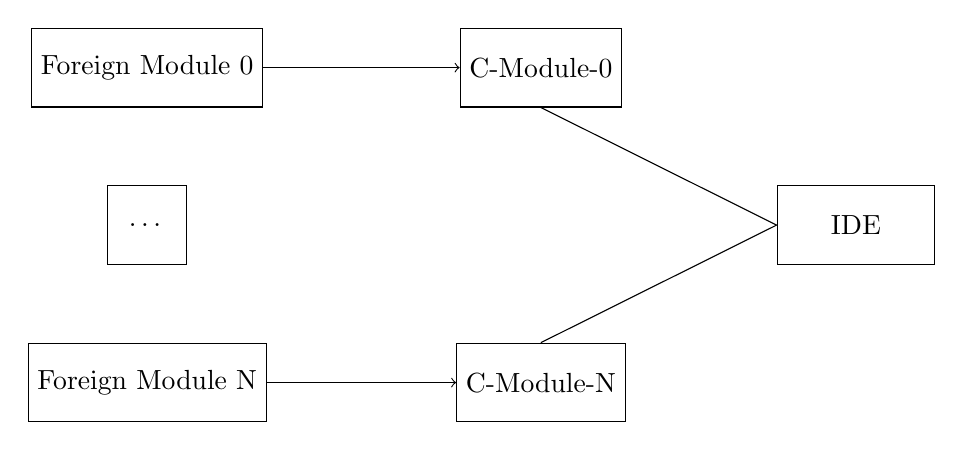
\begin{tikzpicture}
  % Nodes
  \node (p-0) [rectangle, draw, minimum height=1cm, minimum width=2cm] at (-6, 2) {Foreign Module 0};
  \node (dots) [rectangle, draw, minimum height=1cm, minimum width=1cm] at (-6, 0) {\dots};
  \node (p-n) [rectangle, draw, minimum height=1cm, minimum width=2cm] at (-6, -2) {Foreign Module N};
  \node (m-1) [rectangle, draw, minimum height=1cm, minimum width=2cm] at (-1, 2) {C-Module-0};
  \node (m-n) [rectangle, draw, minimum height=1cm, minimum width=2cm] at (-1, -2) {C-Module-N};
  \node (i) [rectangle, draw, minimum height=1cm, minimum width=2cm] at (3, 0) {IDE};
  % Arrow
  \draw (m-1.south) -- (i.west);

  \draw (m-n.north) -- (i.west);

  \draw[->] (p-0) -- (m-1);
  \draw[->] (p-n) -- (m-n);
\end{tikzpicture}

  \end{center}
  \label{fig:fm2}
\end{figure}

This module could be a singular one, acting as a translator, translating the
data flowing between the core and foreign-modules as shown in figure
\ref{fig:fm1}, or each foreign-module could have their own translator as shown
in figure \ref{fig:fm2}.

\subsubsection{Existing Third Party Libraries}

You can use existing JavaScript libraries.

This fascilitates designing modules, as a module could simply act as a binding
between the existing JavaScript library, and the core application. Since the
core application is designed to be an \gls{ide}, one could use existing
JavaScript libraries, like \textit{Monaco}, which is the text editor used by
Visual Studio Code. It comes with an integrated \gls{lsp}-client, which would
enable the application to easily support existing popular languages.

However, being a zero core application, this application could be anything, from
a audio editing program, to a game emulator. Simply using the \textit{JS-DOS}
library, would allow the application to run Doom.

\subsection{IDE User}

Something-something compiled/runtime modules.

As mentioned in chapter \ref{cha:background}, modern \gls{ide}s come with an
integrated module architecture. Which is used to extend/change the \gls{ide},
from as simple as to change the theme, to more drastic changes, like changing
all keybinds to \textit{vim-motions}. In any case, a user expects certain
functionality to already exist in an \gls{ide}, like text editing. A maintainer
of a zero core \gls{ide} could supply modules added at compile time, meaning the
expected functionality is there out of the box, while more thematic modules
could be supplied as runtime modules.

\subsubsection{Standard User}

Stupid/Lazy.

Most users just want an \gls{ide}, and do not spend, nor want to spend, much
time configuring their \gls{ide}.

\subsubsection{Experienced User}

Stupid/Opinionated.

Most experiences users just want to modify their \gls{ide}, instead of actually
using it.

\subsection{Maintainer}

Stupid/Lazy/Opinionated

To make the maintainer of the core application most comfortable, good
documentation is needed. But how good is documentation if it is not updated
when the code being documented is changed? This is where Rusts doc-test system
comes into play. Any function annotated with a docstring, can contain code
examples. If these code examples are written as Rust code, and use assert
statements, then this code is run, during testing, as if it was an actual test.
Meaning the saying \textit{code is documentation}, is
\textit{documentation is code} in Rust.
